\documentclass[a4paper, oneside, openany, dvipsnames, table, 12pt]{article}
\usepackage[italian,british]{babel}
\usepackage{../../../Template/AFKstyleEng}
\usepackage{hyperref}
\usepackage{amsmath}
\usepackage{verbatim}
\usepackage{pdflscape}
\newcommand{\Titolo}{Developer Manual}

\newcommand{\Gruppo}{TeamAFK}

\newcommand{\Redattori}{Simone Federico Bergamin \newline Olivier Utshudi}

\newcommand{\Verificatori}{}

\newcommand{\pathimg}{../Developer_manual/img/logoAFK.png}

\newcommand{\Approvatore}{}

\newcommand{\Distribuzione}{Prof. Vardanega Tullio \newline Prof. Cardin Riccardo \newline TeamAFK}

\newcommand{\Uso}{External}

\newcommand{\NomeProgetto}{Predire in Grafana}

\newcommand{\Mail}{gruppoafk15@gmail.com}

\newcommand{\Versionedoc}{1.0.0}

\newcommand{\DescrizioneDoc}{Developer manual made by \textit{TeamAFK} for the project \textit{Predire in Grafana}.}

\makeindex

\begin{document}
\frontispiece{}

%------------------ COLORI TABELLE 
\definecolor{pari}{RGB}{255, 207, 158} %{HTML}{E1F5FE} %azzurrino
\definecolor{dispari}{HTML}{FAFAFA} %bianco/grigetto 

%definizione colori per tabelle (tranne copertina)
\definecolor{redafk}{RGB}{255, 133, 51}
\definecolor{grey2}{RGB}{204, 204, 204}
\definecolor{greyRowafk}{RGB}{234, 234, 234}
\definecolor{lastrowcolor}{RGB}{176, 196, 222} %steel blue %{255,165,0} orange %{RGB}{255, 207, 158}
\rowcolors{2}{pari}{dispari}
\renewcommand{\arraystretch}{1.5}

%------------------

\newpage
\section*{Changelog}
\begin{longtable}{c c C{3.5cm} C{4cm} C{3cm}}
		\rowcolor{redafk}
\textcolor{white}{\textbf{Version}} & 
\textcolor{white}{\textbf{Date}} & 
\textcolor{white}{\textbf{Description}} & 
\textcolor{white}{\textbf{Name}} & 
\textcolor{white}{\textbf{Role}}\\
		\endfirsthead
		\rowcolor{redafk}
\textcolor{white}{\textbf{Version}} & 
\textcolor{white}{\textbf{Date}} & 
\textcolor{white}{\textbf{Description}} & 
\textcolor{white}{\textbf{Name}} & 
\textcolor{white}{\textbf{Role}}\\
		\endhead
		1.0.0 & 2020-06-10 & Document approved for RQ & Olivier Utshudi & \textit{Manager}\\
		0.7.0 & 2020-06-04 & Writed and checked section \S 7 - \S A & Davide Zilio \newline Fouad Farid & \textit{Programmer} \newline \textit{Verifier} \\
		0.6.0 & 2020-06-04 & Writed and checked section \S 6  & Simone Federio Bergamin \newline Fouad Farid & \textit{Programmer} \newline \textit{Verifier} \\
		0.4.0 & 2020-06-04 & Writed and checked section \S 5 & Olivier Utshudi \newline Simone Meneghin & \textit{Programmer} \newline \textit{Verifier} \\
		0.3.0 & 2020-06-04 & Writed and checked section \S 4 & Simone Federico Bergamin \newline Simone Meneghin & \textit{Programmer}\newline \textit{Verifier}\\
		0.2.0 & 2020-06-03 & Writed and checked sections \S 2- \S 3 & Olivier Utshudi \newline Simone Meneghin & \textit{Programmer}\newline \textit{Verifier}\\
		0.1.0 & 2020-06-03 & Writed and checked section \S 1 & Simone Federico Bergamin \newline Fouad Farid & \textit{Programmer}\newline \textit{Verifier}
	\end{longtable}

%Didascalia tabelle/immagini (prendono come riferimento la subsection)
\counterwithin{table}{subsection}
\counterwithin{figure}{subsection}
\newpage

%indice, indice figure e indice tabelle
\tableofcontents
\newpage
\listoffigures
\newpage
\listoftables
\newpage

\section{Introduction}
	\subsection{Document's purpose}
	Il manuale dello sviluppatore permette ad ogni sviluppatore che si approcci al prodotto software \emph{"Predire in Grafana"} di assimilare le informazioni principali per poter manutenere e estendere tale prodotto. All'interno del documento verrà descritto il prodotto in modo dettagliato, consentendo allo sviluppatore di ottenere una spiegazione esaustiva necessaria per l'attività che andrà a svolgere.

The developer's manual allows each developer reader to absorb \emph{"Predire in Grafana"}'s product key information to maintain and extend the product itself.
This document describes the product in its totality, giving the developer an exaustive explanation required for his tasks.
	
\subsection{Predire in Grafana’s Purpose}

\emph{"Predire in Grafana"} è un plugin realizzato per la piattaforma open source\glo Grafana che permette di calcolare delle previsioni su un flusso dati. Viene utilizzato un algoritmo addestrato dall'utente, la cui definizione è contenuta in un file in formato JSON\glo, per poter effettuare le previsioni.  Viene fornito un applicativo esterno per l'addestramento degli algoritmi di previsione, attualmente sono implementati gli algoritmi di Support Vector Machine\glo e Regressione Lineare\glo . Nello specifico il plugin monitora i dati in ingresso da un certo flusso, come
per esempio percentuali di utilizzo della memoria o temperatura del processore, e produce delle previsioni che vengono successivamente mostrate attraverso l'interfaccia graficaG di Grafana. Il plugin rimane in esecuzione e riceve continuamente informazioni in ingresso da un flusso di dati. In questo modo gli operatori potranno monitorare eventuali cambiamenti sul flusso dati grazie alla previsione in real time\glo ed intervenire, se necessario, sull'origine del problema. 
 
\emph{"Predire in Grafana"} is a plugin made for Grafana which is an open source\glo platform commonly used to analyze data series. The plugin allows users to predict datas on a stream data. \emph{"Predire in Grafana"} plugin uses a JSON file which contains a trained algorithm definition to get predictions. Users can use an external training tool, which use Machine Learning\glo , to get these JSON' files. At the moment only Support Vector Machine and Linear Regression algorithm are implemented. In more detail input datas, like cpu's usage and cpu's temperature, are constantly monitored to get predictions on the aspect you want to examine. Predictions are shown throght Grafana GUI and continue to be updated after being calculated from datas coming from a database. Thanks to this operators can monitor each process and intervene at the root of the problem whenever neccessary.


\subsection{Glossary}
A fine documento viene riportato nell'appendice un glossario che racchiude al suo interno ciascun termine che necessita di una spiegazione dettagliata per risultare più comprensibile al lettore. Tali termini vengono contrassegnati nel documento con una G a pedice.
 
At the end of the document in the appendix is available a glossary where explanations for new or ambiguous terms can be found. These are marked with a subscript G.

\subsection{References}
\subsubsection{Installation}
\begin{itemize}
	\item \url{https://nodejs.org/en/} (\url{https://nodejs.org/it/});
	\item \url{https://git-scm.com/};
	\item \url{https://www.gitkraken.com/};
	\item \url{https://grafana.com/get};
	\item \url{https://www.jetbrains.com/idea/}.
\end{itemize}
\subsubsection{Technologies}
\begin{itemize}
	\item \url{https://reactjs.org/docs/getting-started.html};
	\item \url{https://grafana.com/docs/grafana/latest/developers/plugins/};
	\item \url{https://www.jetbrains.com/help/idea/eslint.html}.
\end{itemize}
\subsubsection{Legal}
\begin{itemize}
	\item \url{https://www.apache.org/licenses/LICENSE-2.0}.
\end{itemize}

\subsubsection{Informative}
\begin{itemize}
	\item \url{https://en.wikipedia.org/wiki/Linear_regression};
	\item \url{https://en.wikipedia.org/wiki/Support_vector_machine}.
\end{itemize}
	


\newpage
\section{System Requirements}
Here the requirements for use of the product are listed.

\subsection{Minimum Hardware Requirements}
Here the requirements for use of the product are listed.
\begin{itemize}
	\item 2GB of RAM;
	\item 5GB of space on a drive;
	\item Dual core processor.	
\end{itemize}

\subsection{Compatible Operating Systems}
The software was developed and tested on the following:
\begin{itemize}
	\item Windows 10;
	\item MacOS 10.15;
	\item Ubuntu 18, 20.
\end{itemize}

\subsection{Compatible Browsers}
Predire in Grafana can be accessed through the following browsers:
\begin{itemize}
	\item Google Chrome version 58 or newer;
	\item Mozilla Firefox version 54 or newer;
	\item Apple Safari version 10 or newer;
	\item Microsoft Edge version 14 or newer;
	\item Opera version 55 or newer.
\end{itemize}




\newpage
\section{Installation}

\subsection{Instruments installation}

\subsubsection{Node.js installation}
The installation of the runtime JavaScript Node.js can be done by visiting  Node.js page at \url{https://nodejs.org/en/download/}. In this site the developer can download the most suitable version of Node.js for his operative system. For Linux user is also possible to use the package manager provided by the OS\glo and exclusively for \textbf{Ubuntu/Debian} developers can run in terinal this code:\\
\texttt{apt-get install nodejs} \\

\subsubsection{Git installation}
For the installation of the version control system, the developer needs to reach Git site's at \url{https://git-scm.com/downloads}. Inside the 'Download' section are available the links to download the compatible version with his operative system. Also Linux base system  can install Git from their package manager or running from \textbf{Ubuntu/Debian} terminal this line:\\
\texttt{apt-get install git} \\

\subsection{Grafana installation}
Developers can install Grafana by reaching its download page at \url{https://grafana.com/grafana/download}. There they can download compatible version for MacOs, Windows and Linux base system. Furthermore, the most common Unix base systems can install Grafana running terminal lines showed in the same page.

\subsubsection{WEB Grafana execution}

Depending from which OS the developer is working on,the execution of WEB Grafana can be done by:
\begin{itemize}
\item \textbf{Windows}: opening "bin" folder in Grafana installation folder
(it should be xxxxxxxxx), and doubl-clicking the "grafana-server" file;
\item \textbf{Linux and MacOS}: running on terminal the following line:\\
\texttt{systemclt start grafana-server}.
\end{itemize} 
After that, the developer needs to reach the address \url{http://localhost:3000/} through a browser. For the first access, the developer needs to fill the fields username with "admin" and password with "admin", and once he/she is in, he/she will need to register himself/herself into the system for next accesses.

\begin{figure}[H]
\centering

\includegraphics[scale=0.25]{./img/web_grafana_login.png}
\caption{WEB Grafana page at \url{http://localhost:3000}}
\end{figure}
\subsection{Plugin and Tool installation}
The following sections will guide developers to install correctely both Training Tool and Prediction Tool.
\subsubsection{GitHub repository clone}
The developer to clone the GitHub repository needs to open the terminal and choose a folder inside the filesystem with command: \\
\texttt{cd /path/folder}
After in the same location, the developer needs to run on terminal this line:\\
\texttt{git clone https://github.com/teamafkSWE/PredireInGrafana-SW.git}
This code creates the folder that contains the source code of Training Tool and Prediction Plugin.
\paragraph*{Dependency}
The following table contains all the dependency adopted for making the tool and the plugin.
%table

\paragraph*{Developer dependency}







\newpage
\section{System enviroment configuration}
	\subsection{IntelliJ IDEA integrated development environment configuration}
A correct IntelliJ IDEA configuration needs to configure the path system\glo and after that to import an existing project.
	
	\begin{figure}[H]
		\centering
		
\includegraphics[scale=0.70]{../Developer_manual/img/intellijidea_main.jpg}
		\caption{IntelliJ IDEA first execution}
	\end{figure}	

	

	\subsubsection{Path system configuration}
Once you run IntelliJ IDEA move to "Configure" then "Settings"in the lower-right corner. Write "Node.js and NPM" in the search bar and check for the correct settings of fields "Node interpreter" and "Package manager", oherwise update them with the correct paths. 

\begin{figure}[H]
		\centering
		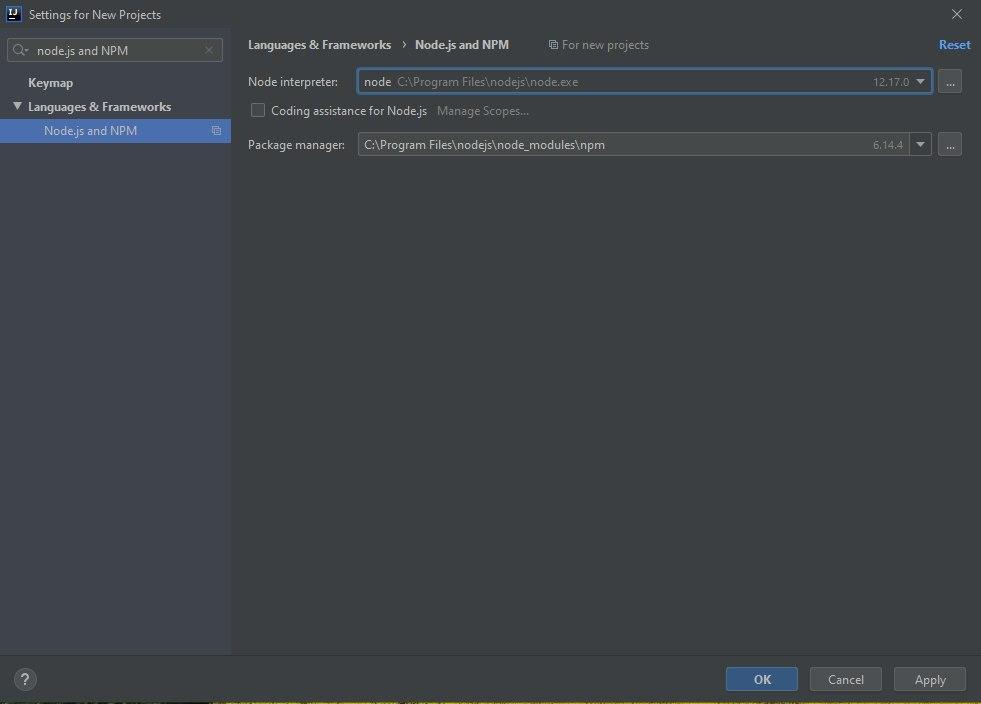
\includegraphics[scale=0.60]{../Developer_manual/img/nodejs_and_npm.jpg}
		\caption{Node.j and NPM settings}
	\end{figure}	

	\subsection{Project import}
From IntelliJ IDEA main window click on "Open or Import" and select the root directory of our project repository folder.

\begin{figure}[H]
		\centering
		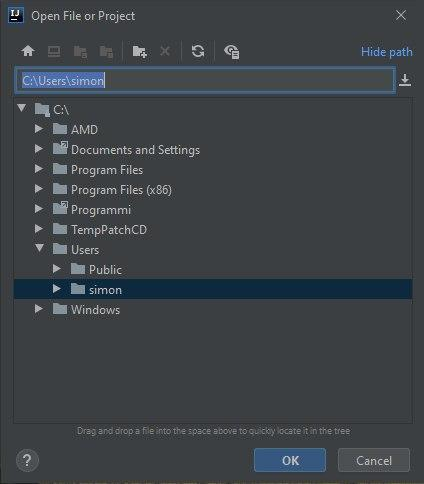
\includegraphics[scale=0.80]{../Developer_manual/img/open_project.jpg}
		\caption{Project path on opening}
	\end{figure}	


	\subsection{ESLint configuration}
		\subsubsection{Automatic configuration}
When ESLint is listed as a dependency in our project IntelliJ IDEA automatically configures it. Move to "File" | "Settings" | "Languages and Frameworks" | "JavaScript" | "Code Quality Tools" | "ESLint" and check that Automatic ESLint configuration option is enabled. 


\begin{figure}[H]
		\centering
		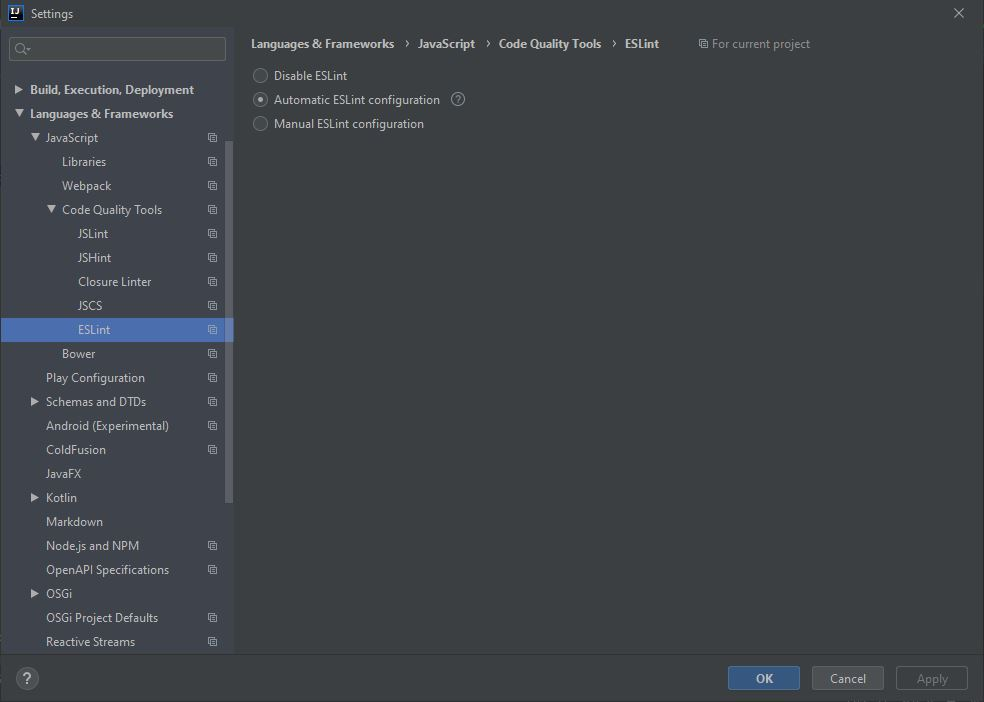
\includegraphics[scale=0.60]{../Developer_manual/img/automatic_eslint_configuration.JPG}
		\caption{Automatic ESLint configuration}
	\end{figure}	

		\subsubsection{Manual configuration}
You can also configure ESLint manually checking the Manual ESLint configuration option and complete fields as it follows:
		\begin{enumerate}
			\item in the "Node Interpreter" field, specify the path to Node.js;
			\item in the "ESLint Package" field, specify the location of the eslint or standard package;
			\item choose the configuration file to use checking "Automatic search" if you want to let IntelliJ IDEA do it for you or specify the file location in the path field;
			\item optionally specify additional command-line options to run ESLint in "Extra ESLint Options" field and specify the location of the files with additional code verification rules in the "Additional Rules Directory" field then confirm the whole configuration.
		\end{enumerate}
		

\begin{figure}[H]
		\centering
		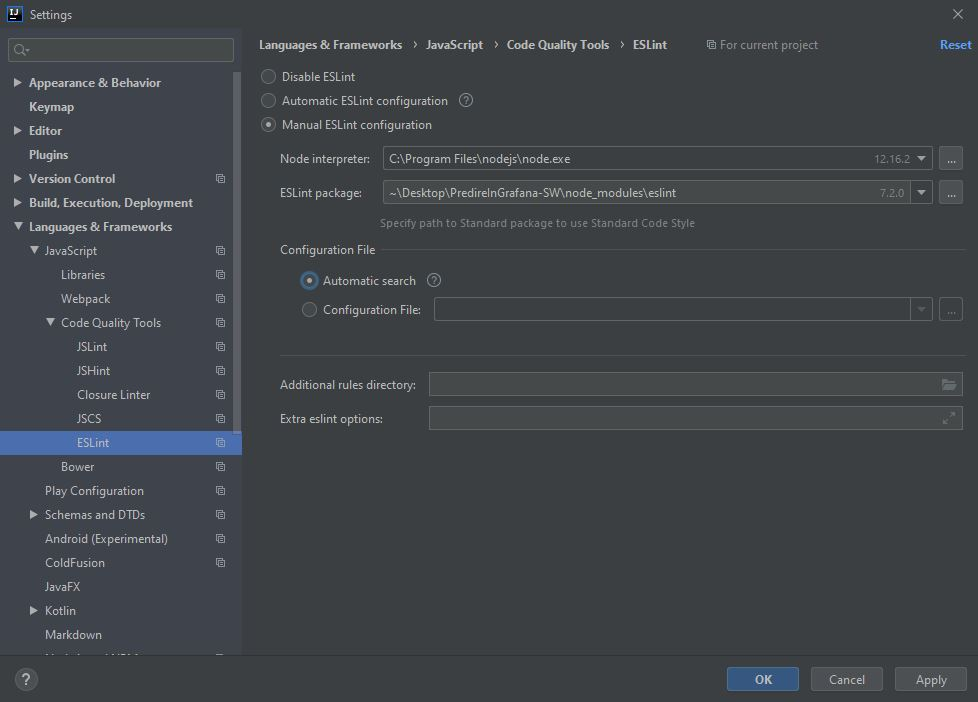
\includegraphics[scale=0.60]{../Developer_manual/img/manual_eslint_configuration.JPG}
		\caption{Manul ESLint configuration}
	\end{figure}	

	
	\subsection{Grafana plugin panel enviroment configuration}
	
	
		\subsubsection{package.json content}
In package.json file you can find all the app informations and requirements needed for its proper functioning. Attributes which represent important information are listed below:
		\begin{itemize}
			\item\textbf{scripts}: it contains all CLI command lines used from the developer: 
				\begin{itemize}
				\item\textbf{build}: this command creates a production-ready build of your plugin. It generates a folder named dist which contains our plugin production files ;
				\newline\texttt{npm run build}
				\item\textbf{test}: this command runs Jest against your codebase (used in automatic tests);
				\newline\texttt{npm run test}
				\item\textbf{dev} : this command creates a development build that's easy to play with and debug using common browser tooling;
				\newline\texttt{npm run dev}
				\item\textbf{watch}: this command run development task in a watch mode.
				\newline\texttt{npm run dev --watch}
			\end{itemize}
			\item\textbf{dependecies}: it contains the following packages needed for our app proper functioning:
			\begin{itemize}
				\item\textbf{@influxdata/influxdb-client}: the reference javascript client for InfluxDB. Both node and browser environments are supported;
    			\item\textbf{axios}: promise based HTTP client for the browser and node.js;
    			\item\textbf{react-files}: a file input (dropzone) management component for React we use when loading JSON files.
			\end{itemize}
			\item\textbf{devDependencies}: it contains the following packages needed for our app proper functioning during development:
			\begin{itemize}
				\item\textbf{@grafana/data}: a library containing most of the core functionality and data types used in Grafana.
				\item\textbf{@grafana-toolkit}: a CLI\glo that enables efficient development of Grafana plugins.
				\item\textbf{@grafana/ui}: a library containing the different design components of the Grafana ecosystem;
				\item\textbf{webpack}: used to compile JavaScript modules. Once installed, you can interface with webpack either from its CLI or API.
			\end{itemize}
		\end{itemize}
		
	\subsection{Training tool enviroment configuration}
	
	
		\subsubsection{package.json content}
In package.json file you can find all the app informations and requirements needed for its proper functioning. Attributes which represent important information are listed below:
		\begin{itemize}
			\item\textbf{scripts}: it contains all CLI command lines used from the developer: 
				\begin{itemize}
				\item\textbf{start}: the command runs the app in development mode. Open texttt{http://localhost:3000} to view it in the browser. The page will automatically reload if you make changes to the code. You will see the build errors and lint warnings in the console;
				\newline\texttt{npm start}
				\item\textbf{build}: this command builds the app for production to the build folder. It correctly bundles React in production mode and optimizes the build for the best performance. The build is minified and the filenames include the hashes. In the end our app is ready to be deployed;
				\newline\texttt{npm run build}
				\item\textbf{test}: this command runs the test watcher in an interactive mode. By default, runs tests related to files changed since the last commit.
				\newline\texttt{npm test}
				\item\textbf{eject}: this command will copy all the configuration files and the transitive dependencies into our project as dependencies in package.json ;
				\newline\texttt{npm run eject}
			\end{itemize}
			\item\textbf{dependecies}: it contains the following packages needed for our app proper functioning:
			\begin{itemize}
				\item\textbf{@testing-library/react}: simple and complete React DOM testing utilities that encourage good testing practices. ;
    			\item\textbf{@testing-library/user-event}: simulate user events for react-testing-library;
    			\item\textbf{bootstrap}: sleek, intuitive, and powerful front-end framework for faster and easier web development;
    			\item\textbf{chart.js}: simple yet flexible JavaScript charting for designers and developers;
    			\item\textbf{is-promise}: test whether an object looks like a promises-a+ promise;
    			\item\textbf{libsvm-js}: c++ library that allows to do Support Vector Machine classification and regression;
    			\item\textbf{ml-svm}: Support Vector Machine in Javascript;
    			\item\textbf{react}: JavaScript library for creating user interfaces. The react package contains only the functionality necessary to define React components;
    			\item\textbf{react-bootstrap}: bootsrap components built with React;
				\item\textbf{react-chartjs-2}: React wrapper for Chart.js 2;     			
    			\item\textbf{react-csv-reader}: React component that handles csv file input. It handles file input and returns its content as a matrix;
    			\item\textbf{react-dom}: package that serves as the entry point to the DOM and server renderers for React. It is intended to be paired with the generic React package, which is shipped as react to npm;
    			\item\textbf{react-scripts}: this package includes scripts and configuration used by Create React App;
    			\item\textbf{svm}: is a lightweight implementation of the SMO algorithm to train a binary Support Vector Machine. As this uses the dual formulation, it also supports arbitrary kernels. 
			\end{itemize}
			\item\textbf{devDependencies}: it contains the following packages needed for our app proper functioning during development:
			\begin{itemize}
				\item\textbf{@testing-library/jest-dom}: custom jest matchers to test the state of the DOM;
				\item\textbf{csv-parser}: streaming CSV parser that aims for maximum speed as well as compatibility with the csv-spectrum CSV acid test suite. Csv-parser can convert CSV into JSON;
				\item\textbf{eslint-plugin-react-hooks}: this ESLint plugin enforces the Rules of Hooks. It is a part of the Hooks API for React.

			\end{itemize}
		\end{itemize}
		
\newpage
\section{Test}
A unity test is the operation that aims to check the correct execution of functions of a component.
The run tests in this projetct, the developer needs to open the terminal and to move inside the folder of the product that needs to be tested (in this case \texttt{PredireInGrafanaSW/my-plugin} or \texttt{PredireInGrafanaSW/prediction-tool}). Inside the folder, the developer has to run the command \texttt{npm run test} inside the terminal. 
\subsection{Edit tests}
Inside the project every components need to be tested. For this reason the developer has to name a test with \textbf{<component name>.test.ts}. Doing so a single component can be checked by a single file.
\subsection{Code Coverage}
Code coverage is the percentuage of the project's code that is analised by tests. This operation is made by Coverall which is an external tool linked to the code through the project's repository. So if the developer wants to chek coverage's value, he has to reach the READ.me file inside the GitHub repository at \url{https://github.com/teamafkSWE/PredireInGrafana-SW}. Inside that file there are two badges and the one with the label "coverage" shows the value of code coverage until the last build.
\newpage
\subsection{Technologies}
\subsubsection{ESLint}
ESLint is a plugin used for code static analisys, so it checks for JavaScript syntax errors.

\subsubsection{InfluxDB}
InfluxDB it'an open source time series database which is used to store and manage data insie the Prediction Plugin. 

\subsubsection{NodeJS}
NodeJS it's an runtime environment that execute JavaScript code outside a web browser. NodeJS it's useful for the tool's developing.

\subsubsection{NPM}
NPM or Node Package Manager it's used to manage dependencies and buld automation. All its functionalities are available by the presence of the file package.json. In this project there are two copies of it because each product needs a dedicated package.json file. So tool's configuration and managemant are indipendent from the plugin.

\subsubsection{React}
React it's a JavaScript library for building user interfaces for both plugin and tool.

\subsubsection{JSX}
JSX it's an extension of JavaScript language syntax. This extension helps to create HTML components for the Training Tool.

\subsubsection{TypeScript}
TypeScript it's a JavaScript superset thet provides static tping to the language. Since Grafana actually is based on this language, TypeScript is used to develop the plugin.

\subsubsection{JSON}
JSON it's an open standard file format used to store the traing data obtained from the Training Tool. So JSON files allows to pass data between tool and plugin.

\subsubsection{CSV}
CSV it's a file format used to store data for plugin's tests.

\subsubsection{Travi CI}
Travis i is an hosted continuous integration servce used to build and test software hosted on GitHub.

\subsubsection{Linear Regression}
The Linear regression it's a linear approch to modeling the relationship between dependent and indipendet variable through points setted on a plan.

\subsubsection{Suport Vector Machine}
A Support Vector Machine it's a supervised learnig model used in machine learning. With a SVM input data thatt are analised  and classified in two different classes.
 
\newpage
\section{Product architecture}
Our product consists of a plug-in developed for the Grafana platform and a Training Tool external to this platform. Therefore the analysis of the architecture is divided into these two components.

\subsection{Training tool}
The Training tool deals with training an SVM or LR algorithm using a dataset inserted by the user, to then generate a JSON file containing the necessary information to perform the prediction. This module has been developed following the \textit{MVVM} behavioral design pattern.

\subsubsection{Architectural design}
We decided to implement this pattern because React\glo was used to build the component and we believed that this pattern coupled well with the structure of the latter. Moreover, it allows to divide the \textit{Presentation Logic}\glo and the \textit{Business Logic}\glo and it allows to reuse some components in other contexts, without having to change them.

As can be seen in the following figure, we have the View that exchanges information on user interactions with the ViewModel, which in turn transforms them into actions on the data performed by the Model.
The data transition from the View to the Model occurs through the instantiation of the ViewModel inside the View. Through this instance, the ViewModel calls the correct functions when the user interacts with the View. The Model provides functionality for the management of the algorithms through the \texttt{SVMtrain} and \texttt{RLtrain} classes that will be used by the ViewModel. 
Finally there is a communication between Model and View for the constant updating of the latter, thanks to a functionality provided by the Grafana platform.

\begin{figure}[H]
\centering
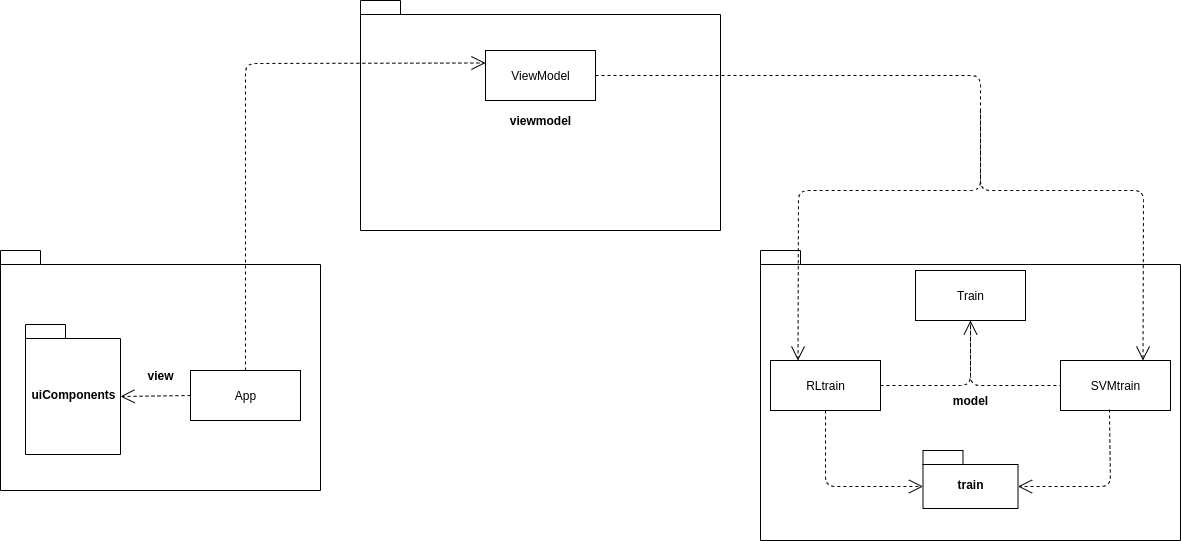
\includegraphics[scale=0.4]{../../../Diagrams/Package_diagrams/tool_design_patern.png}
\caption{Training tool package diagram}
\end{figure}

Analyzing the specific components, our architecture is structured as follows:
\begin{itemize}
\item \textbf{Model}: it manages the \textit{business logic};
\item \textbf{View}: it manages the \textit{presentation logic} through React;
\item \textbf{ViewModel}: it manages the \textit{application logic}\glo. The ViewModel is an abstraction of the View exposing public commands.
\end{itemize}

\subsubsection{Detailed design}

\paragraph{Model}\mbox{} \\ \mbox{} \\
The main component of the Model is the abstract class of the prediction algorithms called Train. Starting with this, we have implemented
two algorithms: Support Vector Machine and Linear Regression.
They are represented respectively by the concrete classes \texttt{SupportSVM}
and \texttt{SupportRL}. We have found that, for families algorithms such as Support Vector Machine and Linear Regression algorithms, it is possible to trace them to a single abstract class as we have provided. 

\paragraph*{Train}\mbox{} \\ \mbox{} \\
The abstract class of the prediction algorithms is called \texttt{Train} and it
represents the contract that all concrete classes must abide to be able to characterize a prediction algorithm. It contains only one parameter: \texttt{algorithm}. The \texttt{train()} method allows you to perform the prediction on a specific dataset. The \texttt{getJSON()} method writes the configuration parameters into the JSON file.

\paragraph*{SupportSVM}\mbox{} \\ \mbox{} \\
To implement the SVM algorithm we developed the concrete class \texttt{SupportSVM}. This class performs the prediction on the dataset. 
It also makes use of components specific to the SVM class imported from the SVM library to perform the real prediction. SupportSVM also contains two fields data: \begin{itemize}
\item \texttt{dataSVM}: reference to the dataset;
\item \texttt{weights}: the weights are the SVM coefficients that will be used to make the prediction.
\end{itemize}
Finally, there is the constructor that allows you to run the method binding to the class.

\paragraph*{SupportRL}\mbox{} \\ \mbox{} \\
To implement the Linear Regression algorithm we developed the concrete class \texttt{SupportRL}. This class performs the prediction on the dataset. It also makes use of components specific to the RL class imported from the RL library to perform the real prediction. SupportRL also contains three fields data: \begin{itemize}
\item \texttt{dataRL}: reference to the dataset;
\item \texttt{numOfX}: the numbers of X founded on the CSV file;
\item \texttt{coefficients}: the coefficients needed to make the prediction.
\end{itemize}
Finally, there is the constructor that allows you to run the method binding to the class.

\begin{figure}[H]
\centering
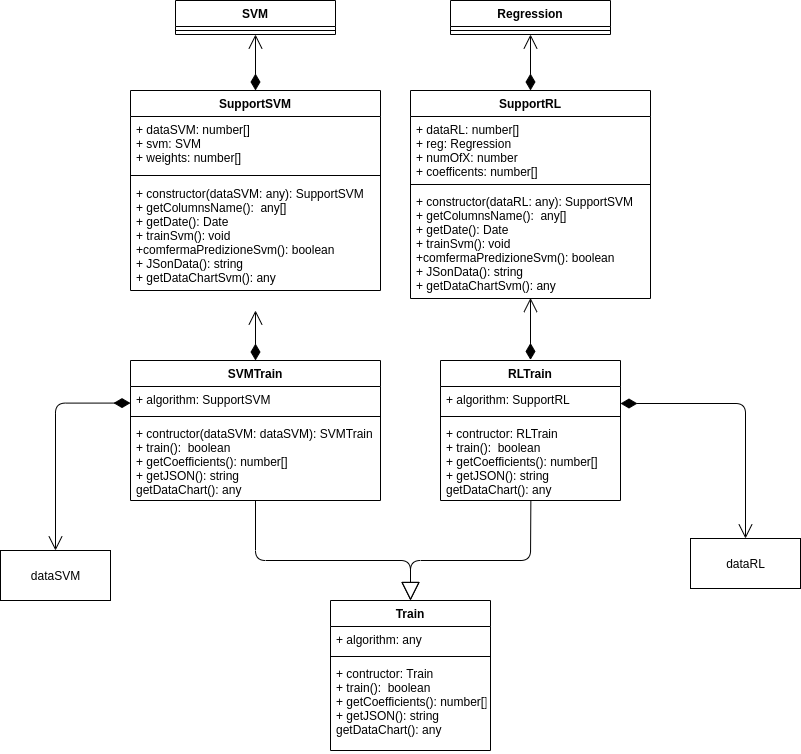
\includegraphics[scale=0.5]{../../../Diagrams/Classes_diagrams/tool_model.png}
\caption{Training tool Model class diagram}
\end{figure}

\paragraph{View}\mbox{} \\ \mbox{} \\
Inside the View there are all the view components.
The \texttt{App} class is the main component and it represents the tool's entry point. Each part of the View has been divided into components and rendered by the App. The communication between these components and the App takes place through the \texttt{props} (conceptually, the components are like JavaScript functions): it accepts arbitrary data (under the name of "props") and returns React elements that describe what should appear on the screen.
Inside there is an instance of the ViewModel for data-binding.

\subparagraph*{App}\mbox{} \\ \mbox{} \\
The \texttt{App} class is the main component and it represents the tool's entry point. Each part of the View has been divided into components and rendered by the App. This class has just one parameter: \texttt{viewModel} is an instance of the ViewModel. The constructor contains the properties in common with the ViewModel. Moreover, it has the following methods:
\begin{itemize}
\item \texttt{changeAlgorithm(event)}: it manages the algorithm user's choice, setting the \\ \texttt{algorithm} state value after the event was made;
\item \texttt{resetAlgorithm(algorithm)}: it sets the \texttt{algorithm} state parameter to the default value;
\item \texttt{setDataFromFile(data, fileInfo)}: it sets the \texttt{data} state parameter and the \\ \texttt{fileName} state parameter with the inserted file's name;
\item \texttt{handleTraining()}: it sends the data to the ViewModel and if the \texttt{performTraining()} method success, it calls the function to write the information into the JSON file, otherwise it resets the algorithm;
\item \texttt{downloadJsonData()}: it creates the DownloadJson component;
\item \texttt{render()}: it creates the InsertCsvButton, ComboBoxAlgorithm, TrainButton and Chart components and it calls the \texttt{downloadJsonData()} function.
\end{itemize}	

\subparagraph*{combo\_box\_algorithm}\mbox{} \\ \mbox{} \\
It renders the combo box for the algorithm's choice.\\
The \texttt{render()} method renders the JSX\glo element wanted.

\subparagraph*{download\_json}\mbox{} \\ \mbox{} \\
It manages and render the "Download" button.\\
The \texttt{downloadJsonFile()} method allow to download the file, making the connection between the browser and the local pc.
The \texttt{render()} method renders the "Download" button.

\subparagraph*{chart}\mbox{} \\ \mbox{} \\
It renders the chart.
This component contains the following parameters: 
\begin{itemize}
\item \texttt{data}: contains the data that must be shown;
\item \texttt{options}: contains the various options that can be applied to the graph, such as colors, axes and the regression line.
\end{itemize}
It also implements the following methods: 
\begin{itemize}
\item \texttt{formatData()}: it associates and manages the data to the graph;
\item \texttt{render()}: it renders the chart graph.

\end{itemize}

\subparagraph*{insert\_csv\_button}\mbox{} \\ \mbox{} \\
It renders the insert button for the CSV file.\\
The \texttt{render()} method renders the "Inserisci file" button.

\subparagraph*{header}\mbox{} \\ \mbox{} \\
It renders the header.\\
The \texttt{render()} method renders the site's header.

\subparagraph*{train\_button}\mbox{} \\ \mbox{} \\
It renders the train button, that will start the training.\\
The \texttt{render()} method renders the "Conferma" button.

\begin{figure}[H]
\centering
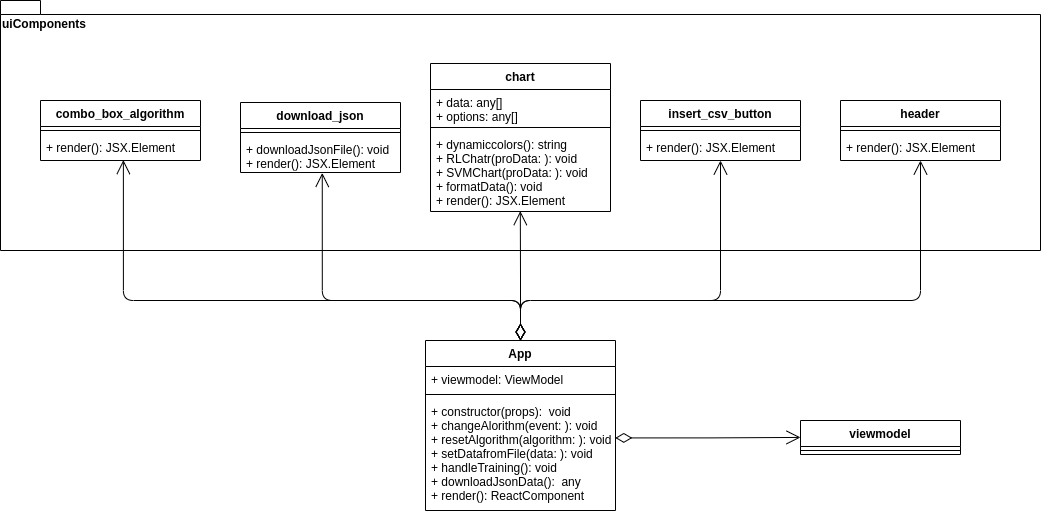
\includegraphics[scale=0.45]{../../../Diagrams/Classes_diagrams/tool_view.png}
\caption{Training tool Model class diagram}
\end{figure}

\paragraph{ViewModel}\mbox{} \\ \mbox{} \\
The data transition from the views to the model occurs through an instance of the ViewModel inside the View. Through this instance, the ViewModel calls the correct functions when the user interacts with the View.
The ViewModel has functions that interact with both the View and the Model (e.g. \texttt{RLChart()} and \texttt{performTraining()}).
To communicate with the Model, there is an \texttt{RLTrain} or \texttt{SVMTrain} instance. In order to instantiate the correct algorithm, the behavioral design pattern Strategy is applied. \\
The ViewModel contains the following variables	: \begin{itemize}
\item \texttt{algorithm}: it contains the string of the chosen algorithm (combo-box component);
\item \texttt{file}: it contains the data of the inserted CSV;
\item \texttt{hasFile}: true if the file CSV has been inserted, false otherwise;
\item \texttt{strategy}: it contains the RLTrain or SVMTrain object.
\end{itemize}

\begin{figure}[H]
\centering
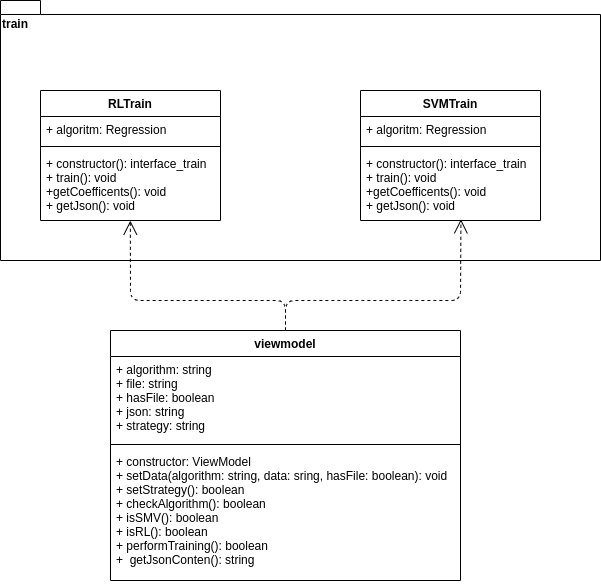
\includegraphics[scale=0.6]{../../../Diagrams/Classes_diagrams/tool_modelview.png}
\caption{Training tool Model class diagram}
\end{figure}

\paragraph*{Sequence diagram}\mbox{} \\ \mbox{} \\
To better explain the set of actions performed in order to process the data for
predict algorithms, the following picture illustrate a sequence diagram which examines SVM. The procedure is also indicative for the others algorithms.

\begin{landscape}
\begin{center}
\begin{figure}[H]
\centering
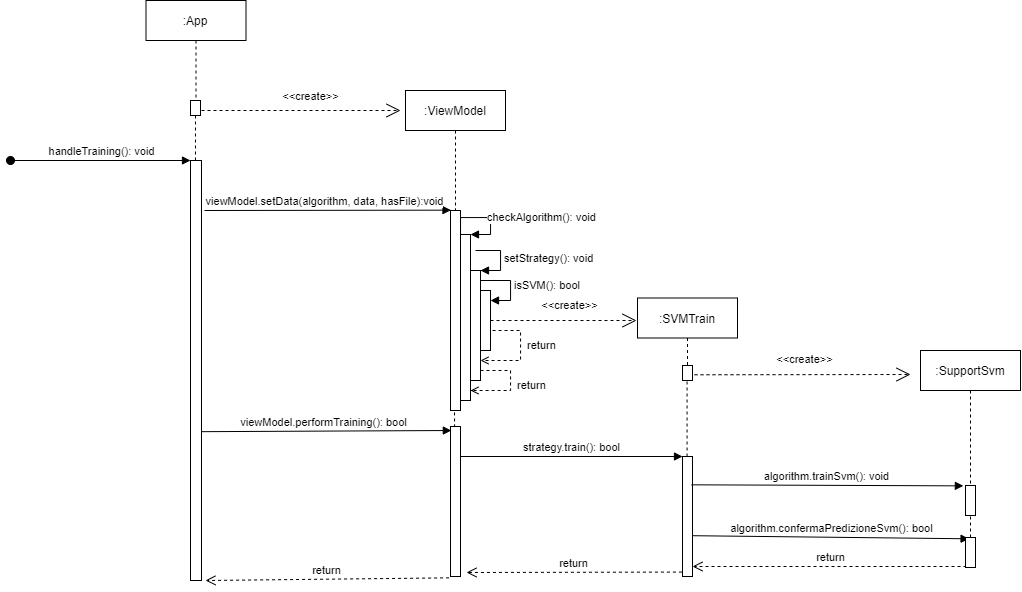
\includegraphics[scale=0.65]{../../../Diagrams/Sequence_diagrams/trainSVM.png}
\caption{TrainSVM sequence diagram}
\end{figure}
\end{center}
\end{landscape}

\subsection{Prediction plug-in}
The Prediction Plug-in will take care of receiving the json input and once the predictors have been connected to a data flow, will allow you to start making calculations forecasting. This module has been developed following the \textit{MVC} design pattern.

\subsubsection{Architectural design}
We felt that this model coupled well with the Grafana plug-in structure.
Moreover, it allows to divide the \textit{presentation logic} and the \textit{business logic} and it allows to reuse some components in other contexts, without having to change them (e.g. the View).
In this module, consisting of several panels within Grafana, the predictor, produced by the external tool, will be associated with the data flow monitored in Grafana. For this module the \textit{MVC} architectural pattern was used. In this architecture the \texttt{Editor} and the \texttt{Panel} share the variable \texttt{props}, instantiated by Grafana.

\begin{figure}[H]
\centering
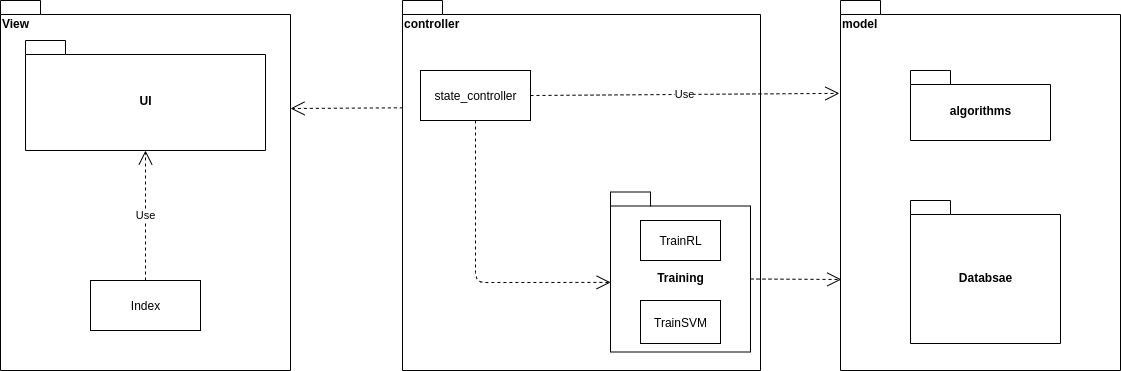
\includegraphics[scale=0.45]{../../../Diagrams/Package_diagrams/plugin_design_pattern.png}
\caption{Prediction plug-in package diagram}
\end{figure}

Analyzing the specific components, our architecture is structured as follows:
\begin{itemize}
\item \textbf{Model}: it manages the \textit{business logic}. It contains
the data prediction algorithms that have been presently implemented and writing the result of the predictions to an Influx database;
\item \textbf{View}: it manages the \textit{presentation logic}. It allows the creation of a customized graphic panel within a Grafana dashboard. With this panel the user can select prediction algorithm settings, incoming data streams and the minimum and maximum thresholds;
\item \textbf{Controller}: it manages the \textit{application logic}. It transforms the data obtained from user interactions and data flows obtained by Grafana in a format suitable for carrying out the actions by the Model.
\end{itemize}


\paragraph{Grafana's role}\mbox{} \\ \mbox{} \\
Grafana plays a fundamental role in the architecture as it allows continuous updating of the View to change the data in the Model. In particular, whenever there are updates on the data in the Model, Grafana makes them available to View through specific methods, together with the configuration of the queries with which this data was obtained. Moreover, through React, it manages the two-way data binding between HTML View and Javascript code, in addition to offering most of the necessary graphic components for the realization of the plug-in View.

\subsubsection{Detailed design}
\paragraph{Model}\mbox{} \\ \mbox{} \\
The Model is the implementation of the \textit{Strategy} pattern. Unlike the tool, in this case the pattern is used to implement the forecast calculation algorithms.
The algorithms are instantiated by the Controller when a JSON file containing the definition of the algorithm to be used is read, therefore extrapolating the values to be passed to the constructors always from the file just inserted.\\
The Model's main component is the interface of the prediction algorithms
called \texttt{Algorithm}. Starting with this, we have implemented
two algorithms: Support Vector Machine and Linear Regression.
They are represented respectively by the concrete classes Svm and Regression. We have found that, for families of Support Vector Machine and Regression algorithms, it is possible to trace them to a single interface as we have provided.

\paragraph*{Algorithm}\mbox{} \\ \mbox{} \\
The interface of the prediction algorithms is called \textit{Algorithm} and it
represents the contract that all concrete classes must abide by
to be able to characterize a prediction algorithm. It contains only one method:
\texttt{predict(input)}. This allows you to perform the prediction on a specific dataset of type \texttt{number}.

\paragraph*{Influx}\mbox{} \\ \mbox{} \\
This class is used to interface and write data to the Influx database WriteInflux. \texttt{Instance} contains an instance of the Influx DB and the \texttt{write()} method writes the data to the Influx database. The "get" methods are used to get informations/parameters helpful to make the connection or specific actions.

\begin{figure}[H]
\centering
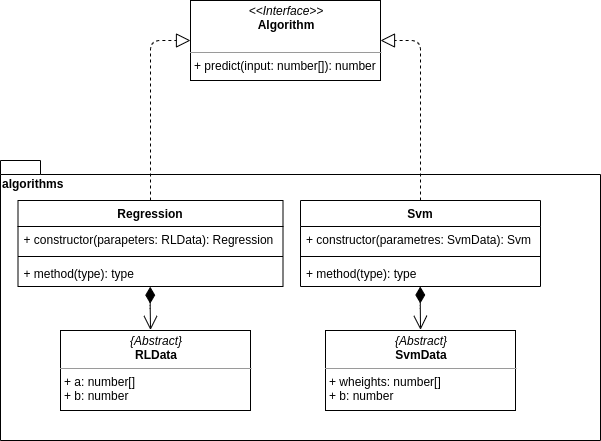
\includegraphics[scale=0.45]{../../../Diagrams/Classes_diagrams/plugin_model.png}
\caption{Prediction plug-in Model class diagram}
\end{figure}

\paragraph{View}\mbox{} \\ \mbox{} \\
The main node of the View is the \texttt{Editor} class, which is the composition of different graphic objects such as CollegamentoView, PrevisioneView, ListaCollegamentiView and CaricamentoJsonView. The latter correspond to the panels and internal objects that will be shown by the plug-in. \\
All these classes are subclasses that extend the React class \texttt{React.PureComponent} which allows you to create components in React:
\begin{itemize}
\item \texttt{CaricamentoJsonView}: it is a view that takes care of loading the JSON file containing the definition of the algorithm previously trained by the training tool;
\item \texttt{CollegamentoView}: this view allows the user to insert a new link, connect a data flow node to the latter and set the thresholds;
\item \texttt{ListaCollegamentiView}: this view lets the user to modify or delete the previous links created;
\item \texttt{PrevisioneView}: this view allows the user to start or stop the monitoring and save the prediction on the Influx database.
\end{itemize}
The \textit{Observer} pattern was used to simplify communication between the Controller and the View components that need to be updated as a result of changing the state of the Controller. In our case the subject class, when it undergoes a status change, it notifies the other components via the \texttt{update()} method.

\begin{figure}[H]
\centering
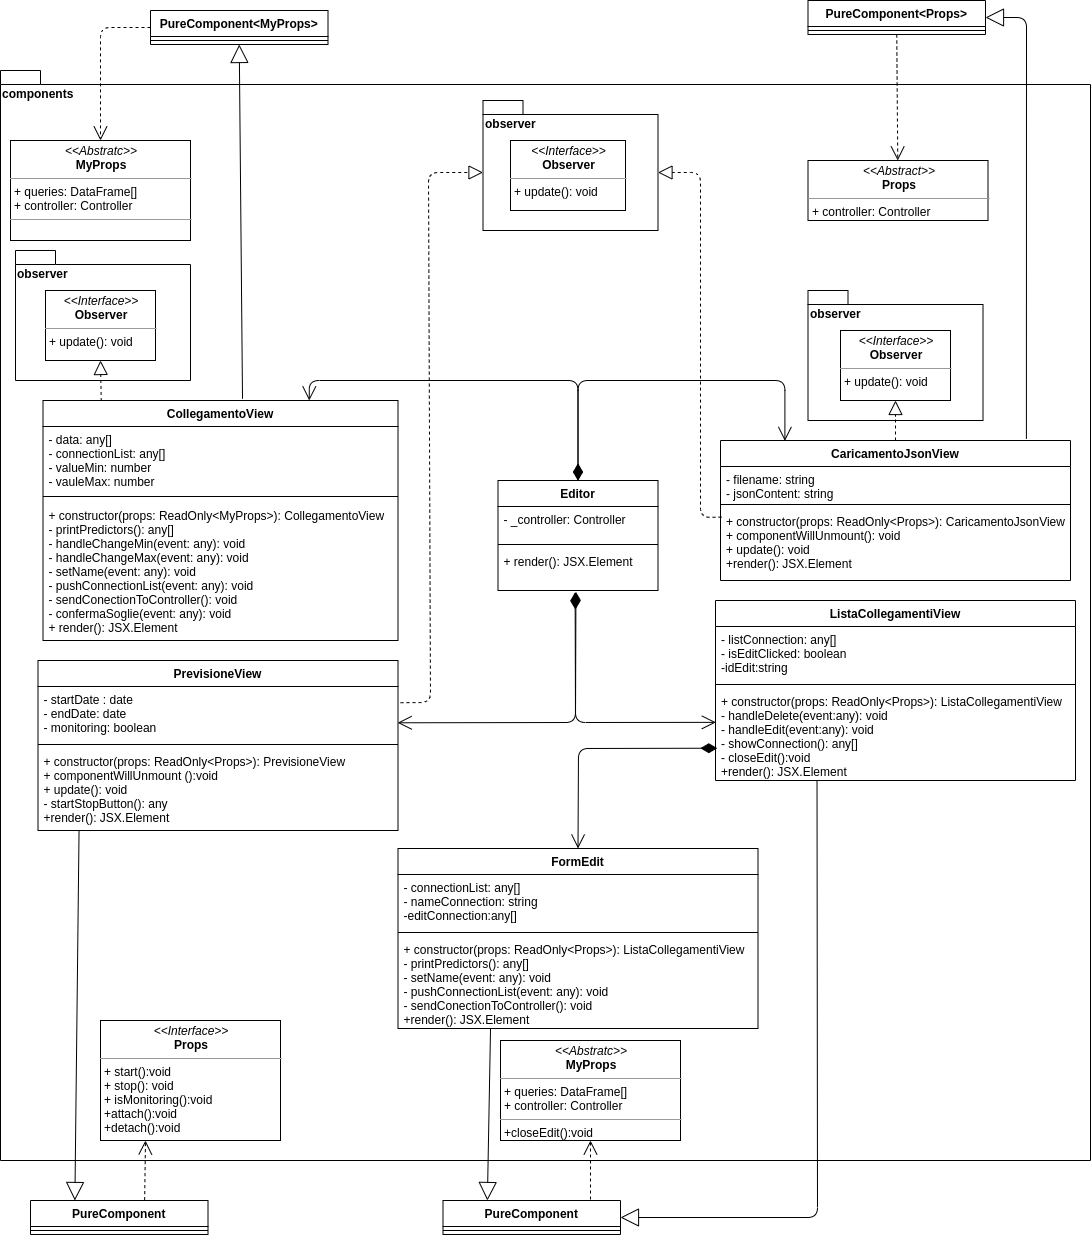
\includegraphics[scale=0.40]{../../../Diagrams/Classes_diagrams/plugin_view.png}
\caption{Prediction plug-in View class diagram}
\end{figure}

\paragraph{Controller}\mbox{} \\ \mbox{} \\
The controller implements the \textit{Observer} pattern; in this case the controller class extends the abstract observable class which therefore represents the subject to be observed, the observer will instead be the view classes.
The Controller will notify the views whenever it changes its state, particularly when the JSON file is inserted and read, when a threshold (\texttt{sogliaMin} and \texttt{sogliaMax}) is set and when the monitoring is started or stopped.\\
When importing the JSON file, the controller will take care of: \begin{itemize}
\item read its contents through the \texttt{setJson(file)} function. Once the Controller finishes reading the file, it notifies the View via the \texttt{update()} method, showing the new information obtained from the file;
\item save a copy of the predictors;
\item apply the correct forecasting algorithm through the \texttt{setStrategy()} method;
\item notify the JSON file upload success views.
\end{itemize}

\begin{figure}[H]
\centering
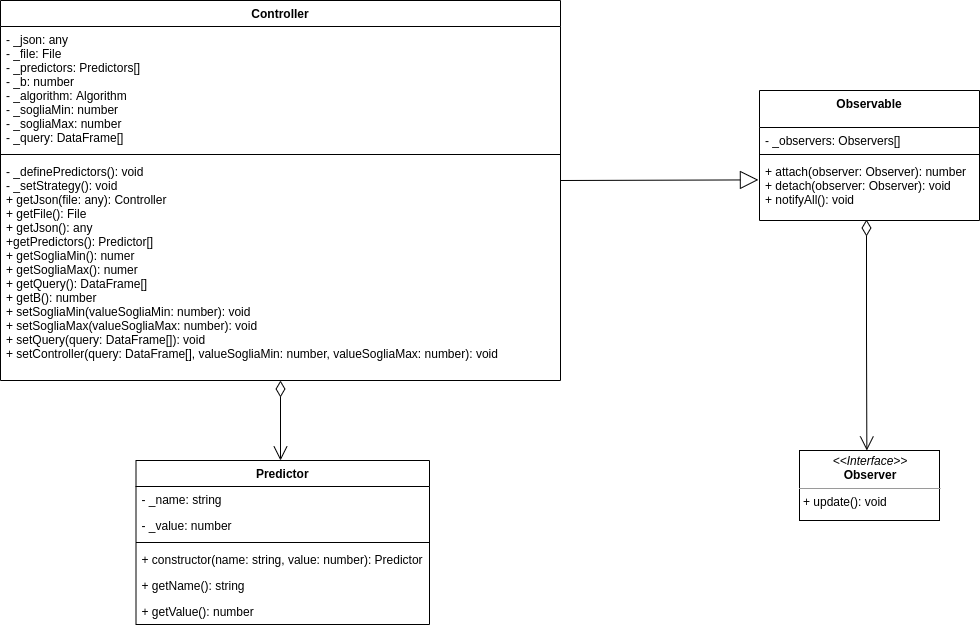
\includegraphics[scale=0.45]{../../../Diagrams/Classes_diagrams/plugin_controller.png}
\caption{Prediction plug-in Controller class diagram}
\end{figure}

\paragraph*{Sequence diagram}\mbox{} \\ \mbox{} \\
The following sequence diagram describes the \texttt{viewGraph()} method, that 
process the data and updates the Grafana's graph with the correct algorithm prediction.

\begin{center}
\begin{figure}[H]
\centering
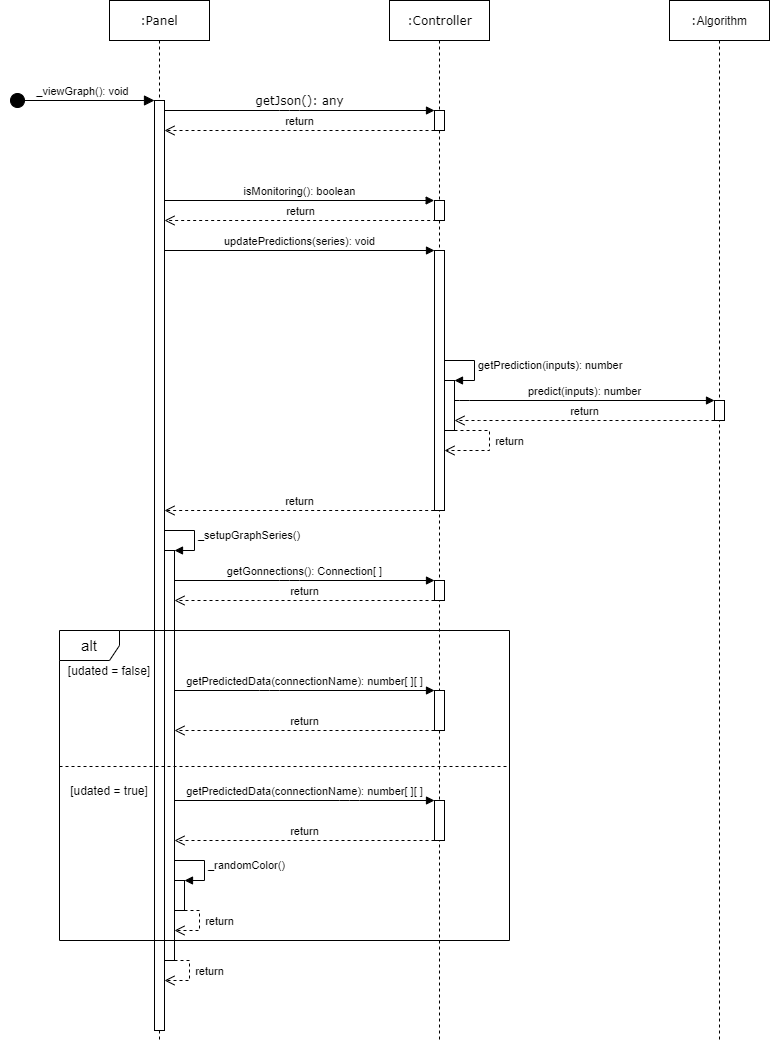
\includegraphics[scale=0.55]{../../../Diagrams/Sequence_diagrams/viewGraph.png}
\caption{\texttt{viewGraph()} sequence diagram}
\end{figure}
\end{center}
\newpage
\section{Product extensibility}
\subsection{Integration of new prediction algorithm}
With this release the product performs trainings and predictions through Support Vector Machine or Linear Regression. But the product can support new procedures beacuse its architecture allows to extend the list of algorithm avaiable by following some steps.\\
Inside Training Tool:
\begin{itemize}
\item in \textit{model}'s \textit{library} package, the developer has to implement the effective algorithm;
\item in \textit{model}'s \textit{train} package the developer has to implement a support class;
\item the developer has to extend the abstract class \textit{Train} located in \textit{model} package, and has to implement the all abstract methods. Then the developer has to import the class inside the \textit{viewmodel}.
\end{itemize}
Inside Prediction Plugin:
\begin{itemize}
\item inside the \textit{model} package, the developer has to extend the class \textit{algorithm}, which is the base for the prediction operation.
\end{itemize}

\newpage
\section{File structure}
	\subsection{JSON file structure}
JSON files which contain trained algorithm definition must be structured as it follow.	

		\subsubsection{Linear Regression}
		\begin{itemize}
			\item\textbf{author}: the file's author. Set in defaul as "TeamAFK";
			\item\textbf{version}: the training tool application version. Set in deafult as "1.0.0";
			\item\textbf{algorithm}: the trained algorithm . Set in default as "Linear Regression"; 	
			\item\textbf{date}: the current date when file is created;
			\item\textbf{predictors}: list of all predictors' labels. These labels are taken from CSV files.
			\item\textbf{result}: list of obtained coefficients from the training. In detail:
			\begin{itemize}
					\item\textbf{a}: list of coefficients values of the regression line formula;
					\item\textbf{b}: bias of the regression line formula;
				\end{itemize}
			\item\textbf{line}: regression line formula;
					
		\end{itemize}
		
		\begin{figure}[H]
		\centering
		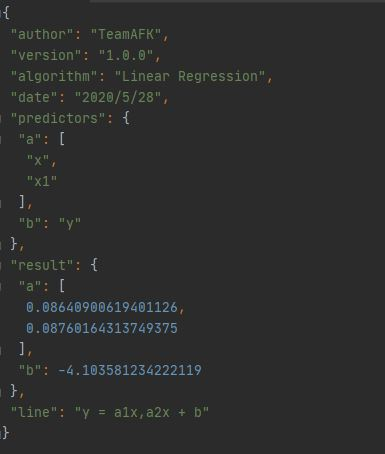
\includegraphics[scale=0.70]{../Developer_manual/img/linear_regression_json.jpg}
		\caption{Example of Linear Regression JSON file}
	\end{figure}	
	
		\subsubsection{Support Vector Machine}
		\subsubsection{Linear Regression}
		\begin{itemize}
			\item\textbf{author}: the file's author. Set in defaul as "TeamAFK";
			\item\textbf{version}: the training tool application version. Set in deafult as "1.0.0";
			\item\textbf{algorithm}: the trained algorithm . Set in default as "SVM"; 	
			\item\textbf{date}: the current date when file is created;
			\item\textbf{predictors}: list of all predictors' labels. These labels are taken from CSV files.
			\item\textbf{result}: list of obtained coefficients from the training. In detail:
				\begin{itemize}
					\item\textbf{a}: list of weights values of the regression line formula;
					\item\textbf{b}: bias of the regression line formula;
				\end{itemize}
			\item\textbf{line}: separation line formula.
					
		\end{itemize}
		
		\begin{figure}[H]
		\centering
		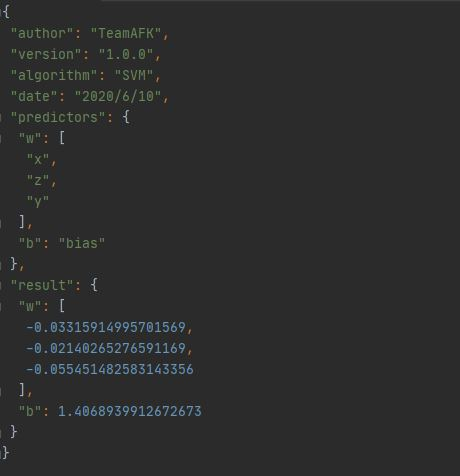
\includegraphics[scale=0.70]{../Developer_manual/img/support_vector_machine_json.jpg}
		\caption{Example of Linear Regression JSON file}
	\end{figure}	
		
	
	\subsection{CSV file structure}
Weather you use choose to train one algorithm intead of another one CSV file has a common structure:
	\begin{itemize}
		\item\textbf{first columns till y column}: each column represents a predictor;
		\item\textbf{y}: this column contains the results.	
	\end{itemize}	 

First line of CSV files must contain predictors tags while the other lines contain values. If you want to add a predictor you must insert a column, before y column, with the predictor tag as first line.

\begin{figure}[H]
		\centering
		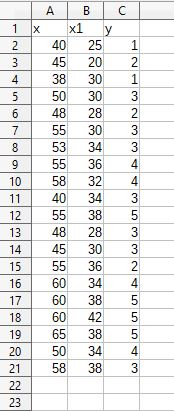
\includegraphics[scale=0.70]{../Developer_manual/img/linear_regression_csv.jpg}
		\caption{Example of Linear Regression CSV file}
	\end{figure}

In SVM CSV files you can find one more column named "label" which contains the data group. 

\begin{figure}[H]
		\centering
		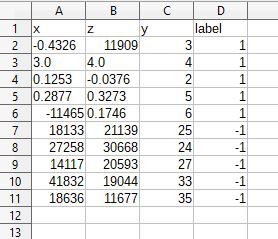
\includegraphics[scale=0.70]{../Developer_manual/img/support_vector_machine_csv.jpg}
		\caption{Example of Linear Regression CSV file}
	\end{figure}
 




\newpage
\appendix
\section{Glossary}

{\Large\textbf{A}\par}
\textbf{Application Logic}\\
Application Logic is any logic that is specific to some application

{\Large\textbf{B}\par}
\textbf{Business Logic}\\
It is the processing logic, in the form of source code, which manages the communication between a user interface and a database. It therefore contains the information that defines or they bind the way a company operates.

{\Large\textbf{C}\par}
\textbf{CSV}\\
CSV (comma-separated values) is a simple file format used to store tabular data, such as a spreadsheet or database.

{\Large\textbf{D}\par}
\textbf{DOM}\\
The Document Object Model (DOM) is a platform and language-neutral interface that allows programs and scripts to dynamically access and update the content, structure, and style of a document.

{\Large\textbf{L}\par}
\textbf{Linear Regression (LR)}\\
Linear regression (LR) is a linear approach to modeling the relationship between a scalar response (or dependent variable) and one or more explanatory variables (or independent variables). The case of one explanatory variable is called simple linear regression.

{\Large\textbf{G}\par}
\textbf{Grafana}\\
Grafana is a multi-platform open source analytics and interactive visualization web application. It provides charts, graphs, and alerts for the web when connected to supported data sources. It is expandable through a plug-in system. End users can create complex monitoring dashboards using interactive query builders.

\textbf{GUI}\\
A graphical user interface (GUI) is an interface through which a user interacts with electronic devices such as computers, hand-held devices and other appliances. 

{\Large\textbf{J}\par}
\textbf{JavaScript}\\
JS is a programming language that conforms to the ECMAScript specification. JavaScript is high-level, often just-in-time compiled, and multi-paradigm. 

\textbf{JSON}\\
JSON (JavaScript Object Notation) is a lightweight data-interchange format. It is easy for machines to parse and generate.

\textbf{JSX}\\
JSX is an extension of the JavaScript language based on ES6, and is translated into regular JavaScript at runtime.

{\Large\textbf{M}\par}
\textbf{Machine learning}\\
Machine learning (ML) is the study of computer algorithms that improve automatically through experience. Machine learning algorithms, such as LR or SVM, build a mathematical model based on sample data, known as "training data", in order to make predictions or decisions without being explicitly programmed to do so.

{\Large\textbf{N}\par}
\textbf{Node.js}\\
Node.js is an open-source, cross-platform, JavaScript runtime environment that executes JavaScript code outside a web browser. Node.js lets developers use JavaScript to write command line tools and for server-side scripts to produce dynamic web page content before the page is sent to the user's web browser.

\textbf{NPM}\\
NPM (Node Package Manager) is a package manager for the JavaScript programming language. It is the default package manager for the JavaScript runtime environment Node.js.

{\Large\textbf{O}\par}
\textbf{OS}\\
An Operating System (OS) is an interface between a computer user and computer hardware. An operating system is a software which performs all the basic tasks like file management, memory management, process management, handling input and output, and controlling peripheral devices.

{\Large\textbf{P}\par}
\textbf{Package}\\
A package (java package) is used to group related classes. They are used to avoid name conflicts, and to write a better maintainable code. 

\textbf{Presentation Logic}\\
The presentation logic of an application is where occurs almost of all interactions with the end user. Manages the reception of user inputs and the presentation of the output of the application to the latter.

{\Large\textbf{R}\par}
\textbf{React}\\
React is a JavaScript library for building user interfaces.

{\Large\textbf{S}\par}
\textbf{Support Vector Machine (SVM)}\\
In machine learning, Support Vector Machines (SVM) are supervised learning models with associated learning algorithms that analyze data used for classification and regression analysis.

{\Large\textbf{T}\par}
\textbf{Typescript}\\
TypeScript is a typed superset of JavaScript that compiles to plain JavaScript.


\newpage

\end{document}